%%
\chapter{Inversion Theories and Algorithm} \label{ch:algorithm}

\section{Introduction}

The inverse problem of this work seeks the solution of a number of
microphysical parameters from observations of different categories. We
thus need to develop an retrieval algorithm that uses statistically
optimized multi-variable fitting, in which the solution sought not
only relies on the presumed classes of potential solutions, but also is in
a continuous space of solutions under statistically formulated criteria
optimizing the error distribution of the retrieval parameters. 
It should be noted that the development of this inversion algorithm 
was built upon our experience with optimization of aerosol emissions 
using the adjoint chemistry transport model (CTM) 
(See Appendix \ref{ch:optems} and \citep{Wang12, Xu13}). 
In essence, the optimization method is consistent  with the adjoint 
modeling  \citep[e.g.,][]{Henze07} that constrains aerosol emissions 
from measurements through inverting a CTM, although 
different physical processes are involved for inversion of AERONET observation. 
Both inversions seek the optimal solutions for a state vector that minimizes 
the differences between the model simulation and observation.

In this chapter, I first present the general theory of inverse problem (section
\ref{sec:invtheory}), covering the Bayesian-based inversion (section
\ref{subsec:map}) and information content analysis
(\ref{subsec:infotheory}). After that in section \ref{sec:algorithm}, 
I describe the key aspects of  designed inversion algorithm: the
definition of the state vector (section \ref{subsec:xy}) and 
considered constraining its \textit{a priori} and smoothness feature 
(section \ref{subsec:ap}), how the state
vector is sought statistically (section \ref{subsec:alg-inv}), how the retrieval 
error is characterized (section \ref{subsec:alg-error}), and quality
control of measurements (section \ref{subsec:alg-qaulity}).


\section{Inversion Theories} \label{sec:invtheory}

\subsection{Maximum a posteriori (MAP) solution of an inverse problem}
\label{subsec:map}

Let $\xbf$ denote a state vector that contains $n$ parameters to be retrieved
(such as PSD parameters and complex indices of refraction), and $\ybf$ an
observation vector with $m$ elements of measurements (such as multi-band
radiances from different viewing angles). Furthermore, let $\Fbf$ indicate a
forward model (such as the radiative transfer model) that describes the
physics of how $\ybf$ and $\xbf$ are related. Then, we have
\begin{equation}
\ybf = \Fbf(\xbf,\bbf) + \epbf\udy
\end{equation}
where the vector $\bbf$ consists of forward model parameters (such as the
surface reflectance) that are not included in $\xbf$ but quantitatively
influence the estimates to our known, and $\epbf\udy$ term is the error that
results from inaccurate modeling and measurement processes. In this
study, we use the best-estimated $\hat{\bbf}$ in the forward model and consider
its contributions to the total measurement accuracy. Linearizing the
forward model at $\bbf=\hat{\bbf}$:
\begin{equation}
\ybf = \Fbf(\xbf,\hat{\bbf})+\hat{\Kbf}\udb(\bbf-\hat{\bbf})+\epbf\udy
\label{eq:mfx-b}
\end{equation}
where $\hat{\Kbf}\udb$ is the weighting function (or Jacobian matrix) 
of the forward model to model parameters $\bbf$ at $\hat{\bbf}$,
$\left.\frac{\partial\Fbf}{\partial\bbf}\right|_{\bbf=\hat{\bbf}}$. 
If we treat the forward model as
linear in the vicinity of the true state of x, the forward model can be
rewritten as:
\begin{equation}
\ybf = \Kbf\xbf + \epbf \label{eq:mfx}
\end{equation}
Where $\epbf$ represents the error that sums the errors from forward modeling
and measurement processes. We only consider the errors propagated from
errors in $\bbf$, but omit any other source in the forward modeling. Thus,
$\epbf=\epbf\udy+\hat{\Kbf}\udb\epbf\udb$, where
$\epbf\udb=\bbf-\hat{\bbf}$ indicates error of $\hat{\bbf}$. $\Kbf$ is the
$m \times n$ Jacobian matrix comprising derivatives of the forward model
with respect to each retrieved parameter,
$\frac{\partial\Fbf}{\partial\xbf}$. 

The inverse problem is to solve $\xbf$ from the measurement $\ybf$ by
inverting the forward model $\Fbf$. In many situations, the forward
model is a complex process with large number of internal uncertainties.
As a result, the inverse problem tends to be an ill-posed problem. In
this regard, the \textit{a priori} constraints are usually considered.
\textit{A priori} represents the knowledge of the state before the
measurement is made. And the true state occurs nearby the \textit{a
priori}:
\begin{equation}
\xbf = \xabf + \epbf\uda. \label{eq:ap}
\end{equation}
where $\xabf$ is the \textit{a priori estimate} and $\epbf\uda$
indicates \textit{a priori} error.

\begin{figure}[t]
  \centering
  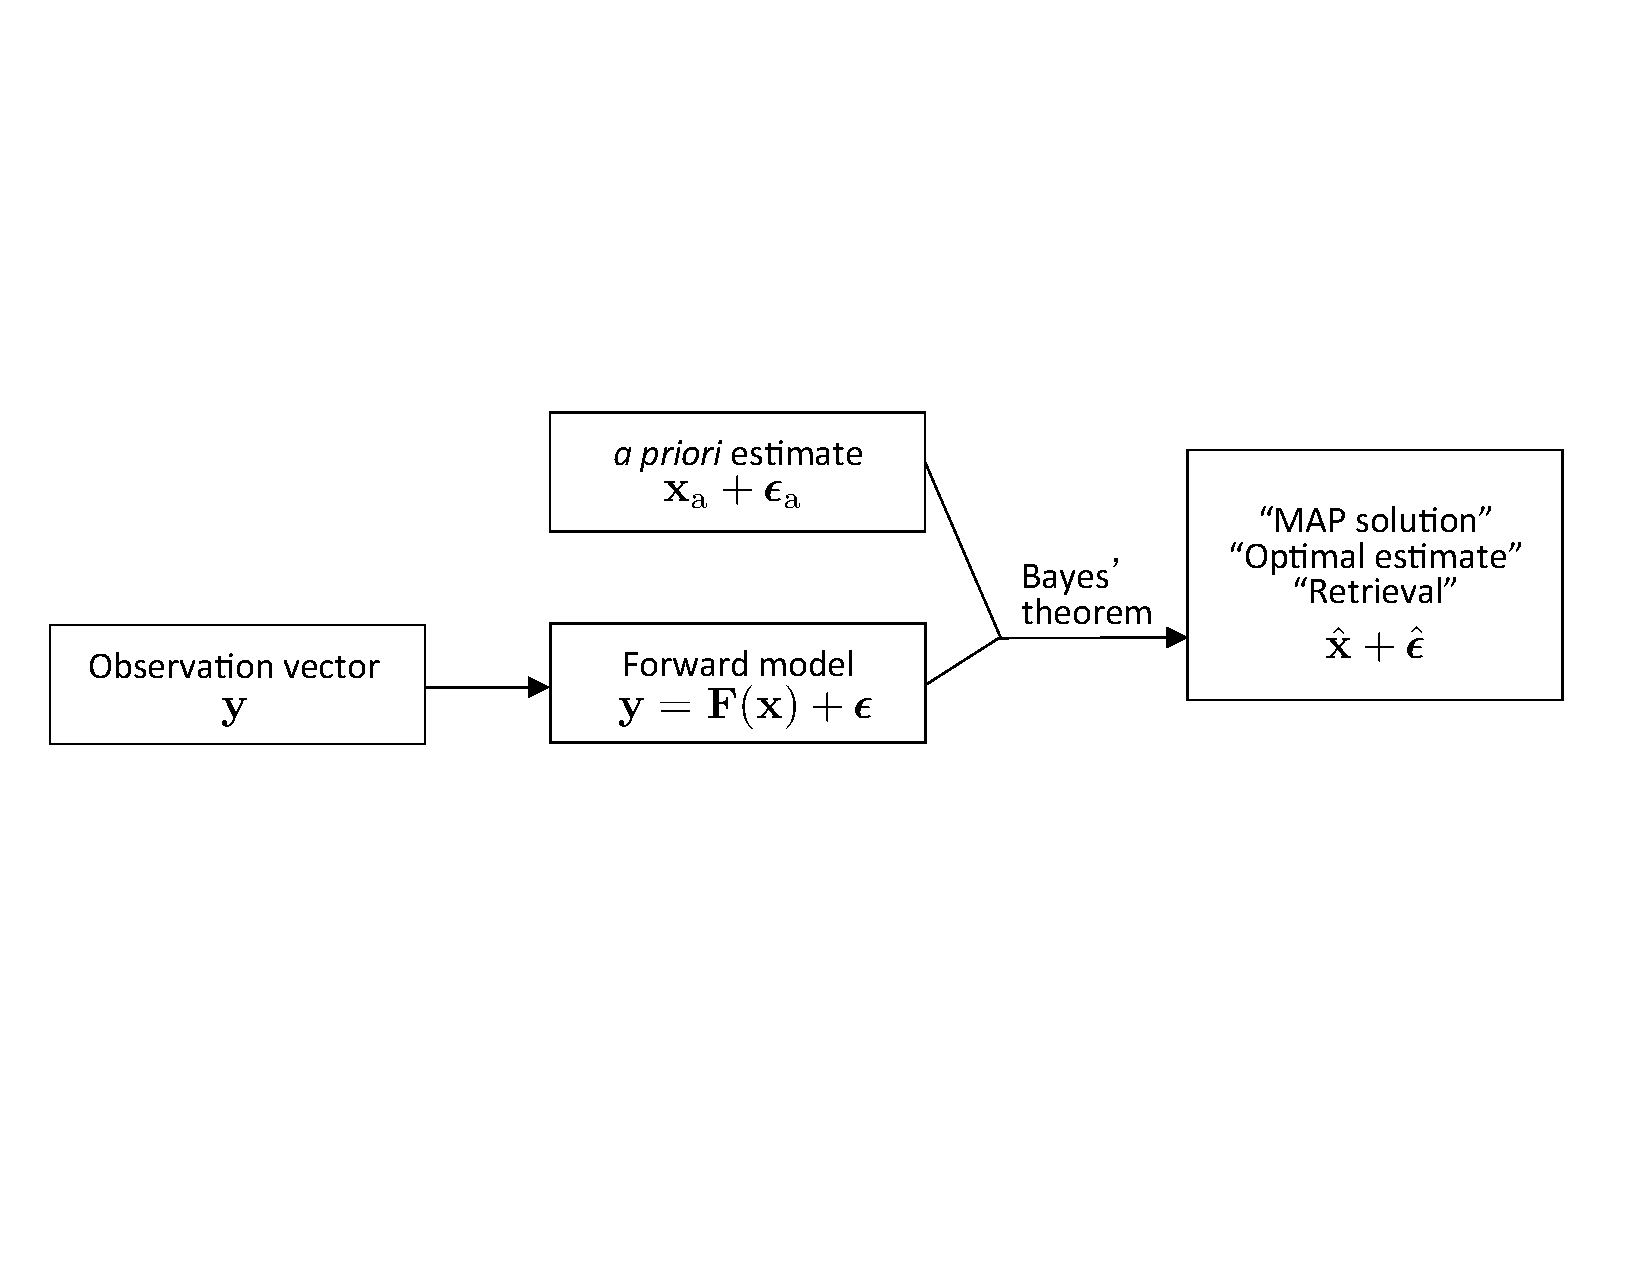
\includegraphics[width={0.9\textwidth}]{figures/MAP.pdf}
  \caption{The concept of an inverse problem that optimzes an estimates
from observations. (Courtesy: Daniel Jacobs)}
  \label{fig:map}
\end{figure}

Then, the inverse problem is solve the equation set (as
illustrated in Figure \ref{fig:map}):
\begin{equation}
\begin{cases}
\ybf = \Kbf\xbf + \epbf \\
\xbf = \xabf + \epbf\uda.
\end{cases}
\label{eq:inverse2}
\end{equation}
Provided that errors of measurements and the \textit{a priori} are characterized
by a Gaussian probability distribution function (PDF) and the forward
model is linear in the vicinity of the true state, the maximum
\textit{a posteriori} (MAP) solution of the state vector, also called the 
retrieval or the \textit{a posteriori} derived with the Bayes's Theorem
is \citep{Rodgers00}:
\begin{equation}
\hat{\xbf} = \xabf + (\Kbf^T\Sbf\udep^{-1}\Kbf+\Sbf\uda^{-1})^{-1}
\Kbf^T\Sbf\udep^{-1}(\ybf-\Kbf\xabf) \label{eq:xhat}
\end{equation}
Here, $\Sbf\uda$ is the error covariance matrix of \textit{a priori},
$\xbf\uda$; $\Sbf\udep$ is the error covariance matrix of the
measurements; $T$ denote matrix transpose operation. 

The "retrieval", $\hat{\xbf}$, in above equation \eqref{eq:xhat}
is corresponding to the maximum posterior
PDF and the minimum of a cost function defined by
\begin{equation}
J = (\ybf-\Kbf\xbf)^T\Sbf\udep^{-1}(\ybf-\Kbf\xbf) +
    (\xbf-\xabf)^T\Sbf\uda^{-1}(\xbf-\xabf).
\label{eq:cost2}
\end{equation} 
J is indeed the negative exponent term of the posterior PDF, which also
follows a Gaussion shape with the expected value of $\hat{\xbf}$ and
the error covariance matrix $\hat{\Sbf}$ given by
\begin{equation}
\hat{\Sbf}^{-1} = \Kbf^T\Sbf\udep^{-1}\Kbf+\Sbf\uda^{-1}. \label{eq:shat}
\end{equation}

$\hat{\Sbf}$ describes the statistical uncertainties in retrieved
$\hat{\xbf}$ due to measurement noise, forward modeling uncertainty, 
and smoothing error \citep{Rodgers00}. The square roots of its 
diagonals are the one-sigma uncertainties of each retrieved parameters 
given the observation uncertainties, forward model uncertainties, 
and prior knowledge of the state. With $\hat{\Sbf}$, we can also 
estimate the uncertainty for any parameter (for example, the aerosol single 
scattering albedo in this study) that can be fully
determined by parameters (for example, aerosol refractive index and PSD
parameters) in $\xbf$ but is not directly retrieved. If one
parameter is a function defined by $\zeta=\zeta{\xbf}$, then the 
uncertainty in derived $\zeta$ is \citep{Rodgers00}:
\begin{equation}
\hat{\epsilon}_\zeta =
\sqrt{\sum_{i=1}^n\sum_{i=1}^n
      \frac{\partial\zeta}{\partial{x_i}} 
      \frac{\partial\zeta}{\partial{x_j}}
      \hat{\Sbf}_{i,j}
      }.\label{eq:zeta}
\end{equation}

\subsection{Information theory} \label{subsec:infotheory}

The Jacobian matrix $\Kbf$ usually serves as gradients in the sensitivity
analysis and can be a useful indicator of information. For a linear
system in the absence of measurement error, the rank of $\Kbf$ indicates
independent pieces of information that can be determined from the
measurements. In practice, error inevitably presents in measurements and
thus can impact the effective rank. To identify the effective
sensitivity of individual measurement to each retrieved parameter, we
define the error-normalized (EN) Jacobian matrix by
\begin{equation}
\tilde{\Kbf} = \Sbf\udep^{-\frac{1}{2}}\Kbf\Sbf\uda^{\frac{1}{2}}
\label{eq:enj}
\end{equation}

$\tilde{\Kbf}$ is also called the ‘pre-whitening’ by \cite{Rodgers00}. 
The superiority of the matrix $\tilde{\Kbf}$ over the matrix $\Kbf$ is 
that it compares the observation error covariance
($\Sbf\udep^{\frac{1}{2}}$) with the natural variability of the
observation vector as expressed by its prior covariance
($\Kbf\Sbf\uda^{\frac{1}{2}}$).
Any component whose natural variability is smaller than the observation
error is not measurable. Therefore, an element $\tilde{\Kbf}_{i,j}$ less than
unity indicates that the measurement component $y_i$ does not contain useful
information for determining parameter $x_j$. In contrast, when
$\tilde{\Kbf}_{i,j}>1$, the larger of its value, the more useful
information retained in $y_i$ for determining $x_j$. Therefore, the
$\tilde{\Kbf}$ matrix provides not only sensitivity of individual 
measurements to each retrieved parameter, but also a capacity-metric 
for those observations to infer retrieved parameters. 

The averaging kernel matrix has been widely used to quantify the
information gained by making a measurement \citep[e.g.,][]{Rodgers98,
Hasekamp05a, Frankenberg12, Sanghavi12}. It provides the sensitivity of 
the retrieval to the true state and is defined by 
\begin{equation}
\Abf=\frac{\partial{\hat{\xbf}}}{\partial\xbf}. 
\end{equation}
Replace $y$ in equation \eqref{eq:xhat} with equation \eqref{eq:mfx}
at $\xbf=\xabf$, 
\begin{equation}
\hat{\xbf} = \xabf + (\Kbf^T\Sbf\udep^{-1}\Kbf+\Sbf\uda^{-1})^{-1}
\Kbf^T\Sbf\udep^{-1}[\Kbf(\xbf-\xabf)+\epbf] 
\end{equation}
Then we have
\begin{equation}
\Abf=\frac{\partial{\hat{\xbf}}}{\partial\xbf}
    =\left(\Kbf^T\Sbf\udep^{-1}\Kbf+\Sbf\uda^{-1}\right)^{-1}
     \Kbf^T\Sbf\udep^{-1}\Kbf
\end{equation}

Matrix $\Abf$ quantifies the ability of the retrieval to infer
$\hat{\xbf}$ given the relationship between $\ybf$ and $\xbf$ (i.e.,
$\Kbf$) and given the observation noise and \textit{a priori} characterization. 
Thus, $\Abf$ represents a perfect retrieval if it is the identity matrix or,
if $\Abf$ is the null matrix, indicates that no information can be gained
from the observations. The trace of $\Abf$ is the
degree of freedom for signal, i.e., $\text{DFS}=\text{Trace}(\Abf)$, 
which represents independent pieces of information that the observation 
can provide. The diagonal elements of the averaging kernel matrix $\Abf$, 
or the DFS components, indicate the partial sensitivity of each 
individual retrieved parameters with respect to their corresponding truth: 
\begin{equation}
\Abf_{i,i}=\frac{\partial\hat{x}_i}{\ptx_i}
\end{equation}
Clearly, $\Abf_{i,i}=1$ indicates that the observation is capable
of fully characterizing the truth of $x_i$; while $\Abf_{i,i}=0$ 
indicates the observation contains zero information on $x_i$ and $x_i$ 
is not measurable. From the formulation of $\hat{\Sbf}$ and $\Abf$, 
we can conclude that only the error covariance and Jacobian matrix, 
but not the retrieval, are important for the purpose of understanding 
information content.

Other quantities used for information analysis of a measurement include
the Shannon information content ($H$) \citep{Shannon48} and the Fisher
information matrix. $H$, a widely used quantity \citep[e.g.,][]{Rodgers98,
Knobelspiesse12}, is defined as the reduction in entropy after 
the measurement
\begin{equation}
H=\frac{1}{2}\ln{|\Sbf\uda|}-\frac{1}{2}\ln{|\hat{\Sbf}|}
 =-\frac{1}{2}\ln{|\hat{\Sbf}\Sbf\uda^{-1}|}
 =-\frac{1}{2}\ln{|\mathbf{I}_n-\Abf|}
\end{equation}
where $\mathbf{I}_n$ is an identity matrix of order $n$. Clearly, 
$H$ is highly related to the DFS for the information analysis. 
In the Gaussian linear case, the Fisher information matrix is equal 
to the inverse of \textit{a posteriori} error covariance matrix, 
$\hat{\Sbf}^{-1}$. The retrieval indeed corresponds to the maximum 
of \textit{a posteriori} PDF and the minimum of retrieval error. It is thus 
straightforward that a higher level of the Fisher information is 
subject to a smaller retrieval error. Due to their close 
relationship with the DFS and $\hat{\Sbf}$, we will not present 
the SIC and Fisher information analysis in this study. 

\section{New Research Algorithm for AERONET Inversion}
\label{sec:algorithm}

Figure \ref{fig:alg} gives an overview of the retrieval algorithm specifically
designed for the analysis and inversion of photo-polarimetric remote
sensing observations, such as those from AERONET. The algorithm builds
upon the UNified and Linearized Vector Radiative Transfer Model
(UNL-VRTM), which consists of seven component modules for the forward
simulation of observations (section \ref{sec:unlvrtm}). The forward 
modeling includes the linearized vector
radiative transfer model (VLIDORT) developed by \citet{Spurr06}, a
linearized Mie code and a linearized T-Matrix code calculating aerosol
single scattering properties \citep{Spurr12}, a module calculating
Rayleigh scattering and a module for gas absorption, plus a surface
model computing bidirectional reflectance/polarization distribution
function (BRDF/BPDF) \citep{Spurr04}. The required input parameters for
the algorithm are the relevant atmospheric profiles (of pressure,
temperature, and gaseous mixing ratio), aerosol loading in terms of AOD
or aerosol columnar volume, aerosol vertical profiles, aerosol
microphysical and chemical parameters (size distribution and complex
refractive index), and surface reflection parameters. The users can
specify up to two modes of the aerosol population. Each mode is
characterized by the total particle number (or volume), the vertical
profile, size distribution, and refractive index. The aerosol-related
modules---Mie, T-matrix, and VLIDORT---are analytically linearized and fully
coupled. Thus, the forward model not only simulates radiance and/or
polarization for a given spectrum, but also simuteneously computes the Jacobians of
these radiation fields with respect to input aerosol microphysical
parameters. Our inversion-oriented UNL-VRTM supplies these Jacobians
together with observation error characterizations and \textit{a priori}
constraints to the statistical optimization procedure for the retrieval.
Objective information content (section \ref{subsec:infotheory}) and 
error analysis (section \ref{subsec:map}) are also included in the
procedure along with the inversion. Although our algorithm is tailored
to measurements from the AERONET SunPhotometer, its modularized
framework enables the simulation and inversion of observations from
various platforms, including satellite sensors. 

\begin{figure}[t]
  \centering
  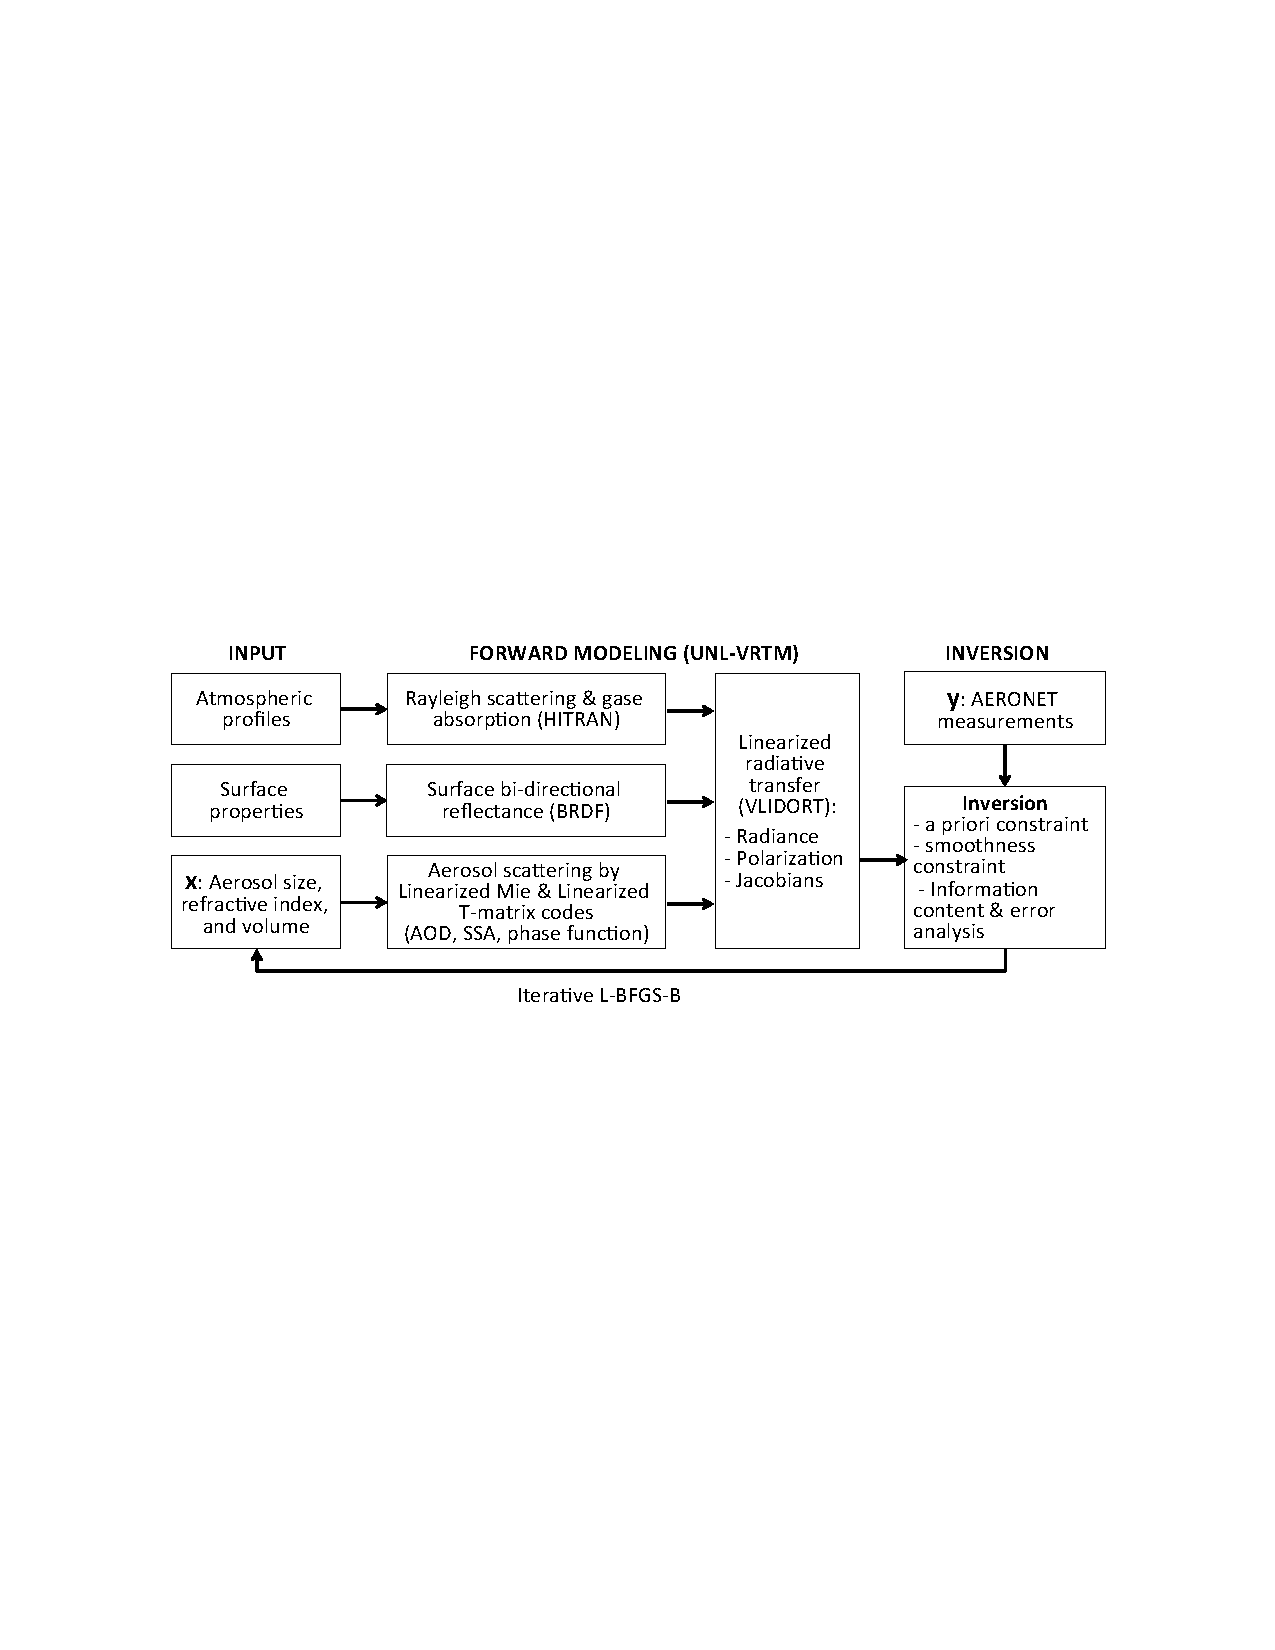
\includegraphics[width={\textwidth}]{figures/algorithm.pdf}
  \caption{General structure of the new research inversion algorithm for
the retrieval of aerosol microphysical parameters from AERONET
photo-polarimetric measurements.}
  \label{fig:alg}
\end{figure}

Development of the inversion component in our algorithm was built upon
our experience with optimization of aerosol emissions using the adjoint
chemistry transport model (CTM) (See Appendix \ref{ch:optems} 
and \citep{Wang12, Xu13}). In essence, the optimization method is 
consistent with the adjoint modeling \citep[e.g.,][]{Henze07}
that constrains aerosol emissions from measurements through inverting a
CTM, although different physical processes are involved for inversion of
AERONET observation. Both inversions seek the optimal solutions for a
state vector that minimizes the differences between the model simulation
and observation. In addition, our algorithm inherits the inversion
strategy from the \Dub algorithm, in particular with regard to
the smoothness constraint on the spectral dependence of the complex
refractive index.

\subsection{Definition of state vector and observation vector}
\label{subsec:xy}

For this study, the observation vector $\ybf$ comprises components from
different sources. As listed in Table \ref{tab:ypars} (and Table
\ref{tab:cimel318} for specific measurements by the SunPhotometer), there are 
four categories of observations, i.e., the direct sun AOD, the sky 
radiance around the solar aureole, the sky radiance in the solar 
principal plane, and the DOLP in the solar principal plane, with 
all measurements performed at 440, 675, 870, and 1020 nm. 
Also indicated in Table \ref{tab:ypars} are the calibration 
errors and other measurement uncertainties that make of the term $\epbf$. 

%% Table 
\begin{table}[t]
  \centering
  \small
  \caption{AERONET observation characteristics.}
  \label{tab:ypars}
  \begin{tabular}{p{3em} p{13em} p{5em} p{13em} }
    \toprule
       Symbol & Parameter & Instrumental uncertainty & Other
uncertainties \\
    \midrule
       $\ybf_1$ & Direct sun AOD & 0.01--0.02 & $\sim$0.02
spatial/temporal variation \\ 
       $\ybf_2$ & Sky radiance in solar almucantar & 5\% & Surface BRDF
and BPDF \\
       $\ybf_3$ & Sky radiance in principal plane & 5\% & Surface BRDF
and BPDF \\
       $\ybf_4$ & DOLP in principal plane & 0.01 & Surface BRDF
and BPDF \\
    \bottomrule
  \end{tabular}
\end{table}

The state vector $x$ contains 11 pairs of parameters characterizing
aerosol properties in the fine and the coarse modes, respectively, the
columnar volume concentration $V_0$, the effective radius $\reff$, the
effective variance $\veff$, and the complex refractive index 
$\mreal-\mimag i$ at 440, 675, 870, and 1020 nm (Table \ref{tab:xpars}). $\reff$ and 
$\veff$ are two commonly used size parameters in the aerosol
radiative quantification, because different types of size distribution
function having same values of $\reff$ and $\veff$ possess similar
scattering and absorption properties \citep{Hansen74}. In line
with many studies \citep{Schuster06, Hasekamp05a, Hasekamp07,
Mishchenko07, Waquet09}, we assume the
aerosol PSD follows a bi-modal lognormal function expressed in equation
\eqref{eq:bilognormal}. All parameters include both the fine and coarse
modes and account for a total of 22 elements ($n=22$). 

\subsection{Combine \textit{a priori} and smoothness constraints}
\label{subsec:ap}

\textit{A priori} information describes our knowledge of the state vector
 before measurements are applied, and an \textit{a priori} constraint is 
commonly used to achieve a well-defined stable and physically reasonable 
solution to an ill-posed problem. Usually, \textit{a priori} knowledge comprises 
both a mean state $\xbf\uda$ and its error $\epbf\uda$ (equation
\eqref{eq:ap}). One of the satisfactory sources for the \textit{a
priori} knowledge is a climatology based on historical measurements. For a given
AERONET site, we use the available inversion products that have been
obtained with the \Dub algorithm, for which the \textit{a priori} can be
well characterized by the mean values and standard deviations of each
component in the state vector. At the same time, the \textit{a priori} can also
be determined from other sources if a historical AERONET retrieval is not
available. For example, we could extract aerosol microphysical
climatology from chemistry transport model simulations
\citep[e.g.,][]{Wang10} or from measurements of \textit{in situ} and/or 
even satellite sensors.

%% Table 
\begin{table}[t]
  \centering
  \small
  \caption{State vector elements and associated constraints for
inversion.\textsuperscript{a}}
  \label{tab:xpars}
  \begin{tabular}{p{5em} p{15em} p{5em} p{5em} }
    \toprule
       Symbol & Parameter & \textit{a priori}\newline constraint? & Smoothness
constraint? \\
    \midrule
       $V_0\fine$, $V_0\coarse$ & Columnar volume ($\mu$m$^3\mu$m$^{-2}$) & 
       $\surd$ & \\
       $\reff\fine$, $\reff\coarse$ & Effective radiance ($\mu$m) &
       $\surd$ & \\
       $\veff\fine$, $\veff\coarse$ & Effective variance  & $\surd$ & \\
       $\mathbf{m}_\text{r}\fine$, $\mathbf{m}_\text{r}\coarse$ & 
       Real part refractive index & $\surd$ & $\surd$ \\
       $\mathbf{m}_\text{i}\fine$, $\mathbf{m}_\text{i}\coarse$ &
       Imaginary part refractive index & $\surd$ & $\surd$ \\
    \bottomrule
    \multicolumn{4}{m{35em}}{\textsuperscript{a}The superscripts, 'c' and
'f', respectively denote fine and coarse aerosol modes. Refractive indices
are for spectral wavelengths of 440, 675, 870, and 1020 nm.}
  \end{tabular}
\end{table}

Among those retrieved parameters, the aerosol volumes---$V_0\fine$ and
$V_0\coarse$---are the most variable or uncertain quantities. A reasonable
initial guess for these quantities could speed up the iterative
inversion. Here, we “look up” their initial values from the AOD
measurements at two spectral wavelengths. Given the \textit{a priori}
 information on the aerosol PSD and refractive indices, the aerosol 
extinction efficiency $\qext$ can be obtained for each fine and coarse 
mode with the Mie code. And the AOD is related to the $V_0\fine$ and
$V_0\coarse$ via equation:
\begin{equation}
\taua = \taua\fine + \taua\coarse 
      = \frac{3V_0\fine\qext\fine}{4\reff\fine} +
        \frac{3V_0\coarse\qext\coarse}{4\reff\coarse}. 
\end{equation}
Clearly, applying the above equation to the AODs at any two spectral
wavelengths, we can easily solve $V_0\fine$ and $V_0\coarse$.

For some parameters, the \textit{a priori} estimates may be poorly known, 
but these parameters behave smoothly with no sharp oscillations. For
example, the aerosol refractive index usually does not vary rapidly over
the visible to near-infrared spectral range. In this regard, a
smoothness constraint could be a preferable addition. The technique of
constraining a smooth solution was pioneered by \citet{Phillips62,
Twomey63}, and has been successfully used to retrieve coherent
aerosol size distributions \citep{Dubovik00a} and atmospheric
vertical profiles \citep{Twomey77}. The principle of the smoothness
constraint is to restrain the degree of non-linearity of a certain
physical parameter by limiting the values of its $d$th derivatives:
\begin{equation}
\Gbf\udd+\epbf_\Delta=\pmb{0} \label{eq:smooth}
\end{equation}
where $\Gbf\udd$ is a differential matrix composed of coefficients for
calculating the $d$th derivatives of $\xbf$ with respect to the dependent
variable, and the vector $\epbf_\Delta$ indicates uncertainties in these
derivatives. 

In particular, for constraining the dependence of the spectral
refractive index with wavelength, the matrix $\Gbf\udd$ calculates the $d$th
difference of the refractive index at four wavelengths (440, 675, 870,
and1020 nm). As discussed by \citet{Dubovik00a}, we assume a linear
relationship between the logarithm of the refractive index and the
logarithm of the wavelength: $\mreal \sim \lambda^{-\alpha}$, and
$\mimag \sim \lambda^{-\beta}$. Further, the matrix $\Gbf_1$  for 
the first difference (of either $\mreal$ or $\mimag$ of one mode) 
can be expressed as:
\begingroup
\allowdisplaybreaks
\begin{align}
\Gbf_1 
&= 
\left[
    \begin{array}{ccc}
    1/{\Delta\lambda_1} & 0 & 0 \\
    0 & 1/{\Delta\lambda_2} & 0 \\
    0 & 0 & 1/{\Delta\lambda_3}  
    \end{array} 
\right] 
\left[
    \begin{array}{cccc}
    -1 & 1 & 0 & 0 \\
    0 & -1 & 1 & 0 \\
    0 & 0 & -1 & 1
    \end{array} 
\right] 
\nonumber \\
&= 
\left[
    \begin{array}{cccc}
    -1/{\Delta\lambda_1} & 1/{\Delta\lambda_1} & 0 & 0 \\
    0 & -1/{\Delta\lambda_2} & 1/{\Delta\lambda_2} & 0 \\
    0 & 0 & -1/{\Delta\lambda_3} & 1/{\Delta\lambda_3}
    \end{array} 
\right]
\end{align}
\endgroup
Here, $\Delta\lambda_1$, $\Delta\lambda_2$, and $\Delta\lambda_1$ are
the denominators for the first-order differences in the logarithm, e.g.,
$\Delta\lambda_1=\ln{\frac{675}{440}}$. As to $\epbf_\Delta$, we assume 
errors in first differences of the refractive index following 
\citet{Dubovik00a}, i.e., 0.2 for $\mreal$ and 1.5 for $\mimag$.

Similar to the approach suggested by \citet{Dubovik00a}, we use
multiple \textit{a priori} constrains in the retrieval.  Specifically, 
we combine the \textit{a priori} constraint of equation \eqref{eq:ap} 
and the smoothness constraint of equation \eqref{eq:smooth}; 
our inverse problem is equivalent to solving the following set of three
equations (in contrast to \eqref{eq:inverse2} that has two
equations):
\begin{equation}
\begin{cases}
\ybf = \mfx + \epbf  \\
\xbf = \xabf + \epbf\uda \\
\pmb{0} = \Gbf\udd+\epbf_\Delta.
\end{cases}
\label{eq:inverse3}
\end{equation}

\subsection{Statistical optimized inversion}
\label{subsec:alg-inv}

Under the assumption of Gaussian-distributed errors, the optimized
solution of equation \eqref{eq:inverse3} according to the 
MAP method corresponds to the state vector that minimizes the quadratic cost
function consisting of multiple terms \citep{Dubovik00a, Dubovik04}:
\begin{equation}
J(\xbf) = \pmb{\gamma}\udy[\ybf-\mfx]^T\Sbf\udep^{-1}[\ybf-\mfx] +
          \pmb{\gamma}\uda(\xbf-\xabf)^T\Sbf\uda^{-1}(\xbf-\xabf) +
          \pmb{\gamma}_\Delta\xbf^T\pmb{\Omega}\xbf.
\label{eq:cost3}
\end{equation}
where $\pmb{\Omega}$ is a smoothing matrix related to $\Gbf\udd$ and the 
error covariance matrix $\Sbf_\Delta$ (of the $d$th derivatives of
$\xbf$) by $\pmb{\Omega}=\Gbf\udd^T\Sbf_\Delta^-1\Gbf\udd$. The
vectors $\pmb{\gamma}\udy$, $\pmb{\gamma}\uda$, and 
$\pmb{\gamma}_\Delta$ are regularization parameters. In principle,
the minimization of three-term cost function given by the equation
\eqref{eq:cost3} is conceptually analogous to the minimization of 
bi-component cost functions \eqref{eq:cost2} generally considered 
in the Bayesian approach \citep{Rodgers00}. These three terms on the 
right-hand size of equation \eqref{eq:cost3} represent,
respectively, (1) the total squared fitting error incurred owing to
departures of the model predictions from the observations, (2) the
penalty error incurred owing to departures of the estimates from the a
priori, and (3) the penalty error incurred owing to departures from the
defined smoothness feature. Overall, the minimization of $J(\xbf)$ achieves
the objective of improving the agreement between the model and the
measurements while ensuring that the solution remains within a
reasonable range and degree of smoothness. 

The regularization parameters in the calculation of $J(\xbf)$ act as weights
to balance the fitting error and the penalty errors. Clearly, a good
assignment of $\pmb{\gamma}$ is of crucial importance for the 
statistical optimal solution. High values of $\pmb{\gamma}\uda$ and
$\pmb{\gamma}_\Delta$ can lead to over-smoothing of the
solution with little improvement to the fitting residuals, while low
values minimize the error term at the cost of greatly increasing the
parameter penalty terms. Optimal values of $\pmb{\gamma}$ for two-term 
cost functions can be identified at the corner near the origin of the 
so-called L-curve \citep{Hansen98}. However, such approach is not 
appropriate to the multi-term cost function. In this study, we assume 
equal weights for observational constraint term and combined 
\textit{a priori} constrain terms in the cost function:
\begin{equation}
\pmb{\gamma}\uda=\frac{1}{2}n^{-1}\mathbf{e}, \quad 
\pmb{\gamma}_\Delta=\frac{1}{2}(n_\Delta-d)^{-1}\mathbf{e}, \quad
\pmb{\gamma}\udy=\left<\frac{1}{4m_k}\right>_{k=1,4}
\end{equation}
Here, $d$ is the order of difference, $\mathbf{e}$ is a vector consisting 
of $n$ elements of 1, and $n_\Delta$ is the number of state elements that 
are supplied with smoothness constraints. Values for $\pmb{\gamma}\udy$ 
are chosen to control the fitting residuals for observations of four 
different categories as listed in Table \ref{tab:ypars}. Each group 
comprises the number of $m_k$ observations for $k$ from 1 to 4. 
The corresponding elements of $\pmb{\gamma}\udy$ for the $k$th group
are $\frac{1}{4m_k}$, which means the observation quadratic term is 
normalized by the observation count of each group.

In principle, solving this inverse problem is tantamount to a pure
mathematical minimization procedure. The minimization of $J(\xbf)$
equation \eqref{eq:cost3}  is performed with an iterative 
quasi-Newton optimization approach using the L-BFGS-B algorithm 
\citep{Byrd95, Zhu94}, which offers bounded minimization to ensure 
the solution stays within a physically reasonable range. 
The L-BFGS-B algorithm requires knowledge of $\xabf$ and
$J(\xbf)$, as well as the gradient of $J(\xbf)$ with respect to $\xbf$,
or $\nabla_{\xbf}J$. By linearizing the forward model F(x), we can 
determine $\nabla_{\xbf}J$ by 
\begin{equation}
\nabla_{\xbf}J(\xbf) = 
   \pmb{\gamma}\udy\Kbf^T\Sbf\udep^{-1}[\ybf-\mfx] +
   \pmb{\gamma}\uda\Sbf\uda^{-1}(\xbf-\xabf) +
   \pmb{\gamma}_\Delta\pmb{\Omega}\xbf.
\label{eq:costadj}
\end{equation}
Here, the Jacobian matrix $\Kbf$ is computed analytically by the
UNL-VRTM (section \ref{sec:unlvrtm}) through equations \eqref{eq:adj-i} and 
\eqref{eq:adj-dolp}. At each iteration, improved estimates of the state vector
are implemented and the forward simulation is recalculated. The
convergence criterion to determine the optimal solution is the smallness
of the reduction of $J(\xbf)$ and the norm of $\nabla_{\xbf}J(\xbf)$. 
The iteration stops when the reduction of $J(\xbf)$ is less than 1\% 
within 10 continuous iterations. Then, the optimal solutions are 
identified corresponding to the smallest norm of $\nabla_{\xbf}J(\xbf)$ from 
these 10 last iterations. In addition, to ensure a
physically reasonable solution, we also perform retrieval error
analysis, and impose a practical quality control on real measurements. 

\subsection{Characterizing retrieval error}
\label{subsec:alg-error}

The retrieval without error characterization is of significantly lesser
value. Once the retrieval is achieved, the retrieval error can be
characterized by the \textit{a posteriori} state, and the error analysis 
can be performed in terms of a linearization of the problem around 
the solution $\hat{\xbf}$. We estimate the retrieval error on each 
state vector element using the error covariance matrix of the 
\textit{a posteriori} state:
\begin{equation}
\hat{\Sbf}^{-1} = \hat{\Kbf}^T\Sbf\udep^{-1}\hat{\Kbf}+\Sbf\uda^{-1} +
\pmb{\Omega}. 
\label{eq:shat3}
\end{equation}
where $\hat{\Kbf}$ is the Jacobian matrix of the forward model $\mfx$ 
at the solution $\hat{\xbf}$. It should be noted that the above 
three-term equation of \textit{a posteriori} are formularized 
according to the cost function defined in the 
equation \eqref{eq:cost3}. Simply, the retrieval 
error for each element can be estimated by:
\begin{equation}
\hat{\epsilon}_i=\hat{\Sbf}_{i,i}^{\frac{1}{2}}
\end{equation}
With $\hat{\Sbf}$ applied to equation \eqref{eq:zeta}, we can also estimate
the uncertainty in parameters (such as $\assa$ and asymmetry factor in this
study) that can be fully determined by the parameters in $\xbf$ but are not
themselves directly retrieved.

\subsection{Quality control of measurements}
\label{subsec:alg-qaulity}

We apply a suite of quality criteria to ensure (a) a cloud-free condition,
(b) that aerosol particles are quasi-homogeneously distributed in the
horizontal plane within the scanning region, and (c) the measurements
are densely populated and cover a wide range of scattering angles so
that they provide sufficient information to retrieve all parameters
falling within specified uncertainty levels. More specifically, these
criteria are as follows: (i) the number of AOD observations $\geq$ 2 within a 
$\pm$25-minute centered at the period of a full scan sequence; (ii) sky
radiance observations are excluded when the scattering angle is less
than 3.2$^\circ$ and DOLP observations are excluded when the scattering angle
is smaller than 5$^\circ$; (iii) a symmetry check for the almucantar radiances: the
difference is less than 5\% for the azimuthal angle of 180$^\circ$ and less than
10\% elsewhere; and (iv) principal-plane observations are discarded when
their second derivatives with respect to the scattering angle are beyond
the smoothing threshold. Although most of these criteria follow
\citet{Holben06}, we also check the smoothness of the principal-plane
radiances and DOLP to identify scans that are contaminated by cloud. We
apply the threshold on the second derivative of radiance (or DOLP) with
respect to scattering angle in order to restrain local oscillations of
radiance (or DOLP) caused by clouds or heterogeneous aerosol plumes.
Thus, applying such a threshold can effectively remove sharp kinks and
ensure continuous quantities in the principal-plane scanning sequences. 
Indeed, this smoothness check shares the same principle to the smoothness 
constraint presented in the section \ref{subsec:ap}. 

\section{Acknowledgements}

We thank Daven Henze, Oleg Dubovik, and Brent Holben for constructive
suggestions and useful discussions on the inversion algorithm
developement. This work is supported by a NASA Earth and Space Science
Fellowship and the NASA Radiation Sciences Program and the Glory mission
program. Most content in this chapter also appear in two articles
published on \textit{Journal of Geophysical Research – Atmospheres}
\citep{Xu15a, Xu15b}.
